% This must be in the first 5 lines to tell arXiv to use pdfLaTeX, which is strongly recommended.
\pdfoutput=1
% In particular, the hyperref package requires pdfLaTeX in order to break URLs across lines.

\documentclass[11pt]{article}

% Remove the "review" option to generate the final version.
\usepackage[]{ACL2023}

% Standard package includes
\usepackage{times}
\usepackage{latexsym}

% For proper rendering and hyphenation of words containing Latin characters (including in bib files)
\usepackage[T1]{fontenc}
% For Vietnamese characters
% \usepackage[T5]{fontenc}
% See https://www.latex-project.org/help/documentation/encguide.pdf for other character sets

% This assumes your files are encoded as UTF8
\usepackage[utf8]{inputenc}

% This is not strictly necessary, and may be commented out.
% However, it will improve the layout of the manuscript,
% and will typically save some space.
\usepackage{microtype}

% This is also not strictly necessary, and may be commented out.
% However, it will improve the aesthetics of text in
% the typewriter font.
\usepackage{inconsolata}

\usepackage{graphicx}


% If the title and author information does not fit in the area allocated, uncomment the following
%
%\setlength\titlebox{<dim>}
%
% and set <dim> to something 5cm or larger.

\title{Extractive summarisation of biomedical research articles using TextRank, WordRank, and a hybrid approach}

% Author information can be set in various styles:
% For several authors from the same institution:
% \author{Author 1 \and ... \and Author n \\
%         Address line \\ ... \\ Address line}
% if the names do not fit well on one line use
%         Author 1 \\ {\bf Author 2} \\ ... \\ {\bf Author n} \\
% For authors from different institutions:
% \author{Author 1 \\ Address line \\  ... \\ Address line
%         \And  ... \And
%         Author n \\ Address line \\ ... \\ Address line}
% To start a seperate ``row'' of authors use \AND, as in
% \author{Author 1 \\ Address line \\  ... \\ Address line
%         \AND
%         Author 2 \\ Address line \\ ... \\ Address line \And
%         Author 3 \\ Address line \\ ... \\ Address line}

\author{Kristina Levina \\
  Course code: 732A81 \\
  LiU-ID: krile102 \\}

\begin{document}
\maketitle
\begin{abstract}
This project aims at building a tool to generate a summary of a biomedical research manuscript automatically based on the main text. To this end, extractive summarisation is employed. The motivation behind choosing extractive summarisation is, in essense, the neccessety to preserve key sentences from the main text. Extractive summarisation will retrieve sentences based on their importance without rephrasing them, thereby excluding misinterpretations. The meaning preservation is crucial for scientific texts. In this project, PubMed dataset is used. A subset of 100 articles and their abstracts have been manually looked through and filtered so that articles and abstracts have similar characteristincs in terms of relative number of sentences of the abstract to the main text. As a result, 24 articles and their human-written summaries (abstracts) were selected. Three algorithms were chosen for extractive summarisation: TextRank, WordRank, and their combination. Their performance was assessed using ROUGE (recall), BLEU (precision), and F1 score. The obtained results show that Y better suits for the considered task. 

\end{abstract}

\section{Introduction}

With increasing volume of published articles in medical research, it becomes increasingly difficult for doctors, medical staff, and public health officials to stay updated. Sometimes, a

\section{Theory}
\subsection{PageRank}
\subsection{ROUGE}
\subsection{BLEU}

\section{Data}

Data are taken from the paper by \citet{cohan2018discourse}. This dataset contains a large collection (100,000) of scientific articles from the biomedical domain (OpenAccess PubMed articles). Data are hosted in \href{https://github.com/armancohan/long-summarization}{GitHub}. Each article has the following fields: 
\begin{verbatim}
{ 
  'article_id': str,
  'abstract_text': List[str],
  'article_text': List[str],
  'section_names': List[str],
  'sections': List[List[str]]
}
\end{verbatim}

For this project, I have looked through 100 articles and considered only articles meeting the following assumptions: First, the provided abstract should be between 8\%--12\% of the main text in terms of number of sentences. This is to ensure similar conditions for generating summaries. Second, the number of sentences of the main manuscript text should be larger than 50 to meet the objective of long document summarisation. Out of 100 articles, only 24 met this conditions.

An example of the beginning of one chosen article is as follows:

\texttt{'["anxiety affects quality of life in those living with parkinson \'s disease ( pd ) more so than overall cognitive status , motor deficits , apathy , and depression [ 13 ] .", \'although anxiety and depression are often related and coexist in pd patients , recent research suggests that anxiety rather than depression is the most prominent and prevalent mood disorder in pd [ 5 , 6 ] . yet ,\', }

The beginning of the corresponding summary is as follows:

\texttt{'["<S> research on the implications of anxiety in parkinson \'s disease ( pd ) has been neglected despite its prevalence in nearly 50\% of patients and its negative impact on quality of life . </S>", \'<S> previous reports have noted that neuropsychiatric symptoms impair cognitive performance in pd patients }

The data have been already tokenised. From the abstract text, <S> and </S> tags were removed. Further preprocessing included stop word removal, lemmatisation, and non-alphabetic characters' removal. This preprocessing has been done using the Spacy language model. Stop words were removed to avoid sentence ranking based on common and frequent words rather than important words. Lemmatisation was used to treat same words in an exactly same manner. Non-alphabetic characters were removed to avoid their influence on the ranking results. Punctuation and numerals should not affect the sentence importance.
 


\section{Method}
\subsection{TextRank}
\subsection{WordRank}
\subsection{Hybrid}
\subsection{Evaluation}

\section{Results}

The ROUGE\_1, BLEU\_1, and F1\_1 scores respectively denote ROUGE, BLEU, and F1 scores of unigrams between the human-written and generated summaries. The results are shown in Fig. \ref{fig:uni} and Tables \ref{tab:means} and \ref{tab:mors}. Both TextRank (36.0) and Hybrid80 (35.9) yield high mean F1\_1 scores relative to other algorithms, but considering margin of error, the estimation by Hybrid80 is slightly more robust (35.9 $\pm$ 3.3 versus 36.0 $\pm$ 3.7). Both TextRank (27.0) and Hybrid80 (26.8) yield high mean BLEU\_1 scores, but considering margin of error, again the estimation by Hybrid80 is slightly more robust (26.8 $\pm$ 3.2 versus 27.0 $\pm$ 3.7). WordRank yields the highest ROUGE\_1 score (60.1 $\pm$ 4.1). 

The ROUGE\_2, BLEU\_2, and F1\_2 scores respectively denote the ROUGE, BLEU, and F1 scores of bigrams between the human-written and generated summaries. The results are shown in Fig. \ref{fig:bi} and Tables \ref{tab:means} and \ref{tab:mors}. The ROUGE\_3, BLEU\_3, and F1\_3 scores respectively denote the ROUGE, BLEU, and F1 scores of trigrams between the human-written and generated summaries. The results are shown in Fig. \ref{fig:tri} and Tables \ref{tab:means} and \ref{tab:mors}. TextRank shows the highest values of ROUGE\_2 and ROUGE\_3 (21.2 $\pm$ 4.9 and 10 $\pm$ 3.7, respectively), BLEU\_2 and BLUE\_3 (10.1 $\pm$ 2.7 and 5 $\pm$ 2.0, respectively), and F1\_2 and F1\_3 (13.4 $\pm$ 3.2 and 6.5 $\pm$ 2.5, respectively).

The total running times of all four algorithms for summarisation of 24 data samples is shown in Table \ref{tab:time}. TextRank (1 min) performs 16 times faster than other algorithms (16 min).

\begin{figure}[!h]
\centering
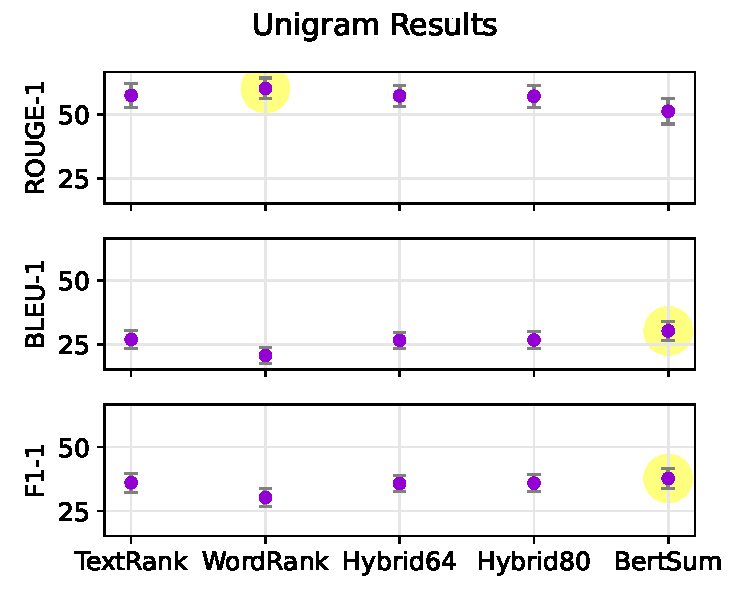
\includegraphics[scale = 0.5]{../figures/unigrams.pdf}
\caption{ROUGE, BLEU, and F1 score of unigrams between the human-written and generated summaries.\label{fig:uni}}
\end{figure}

\begin{figure}[!h]
\centering
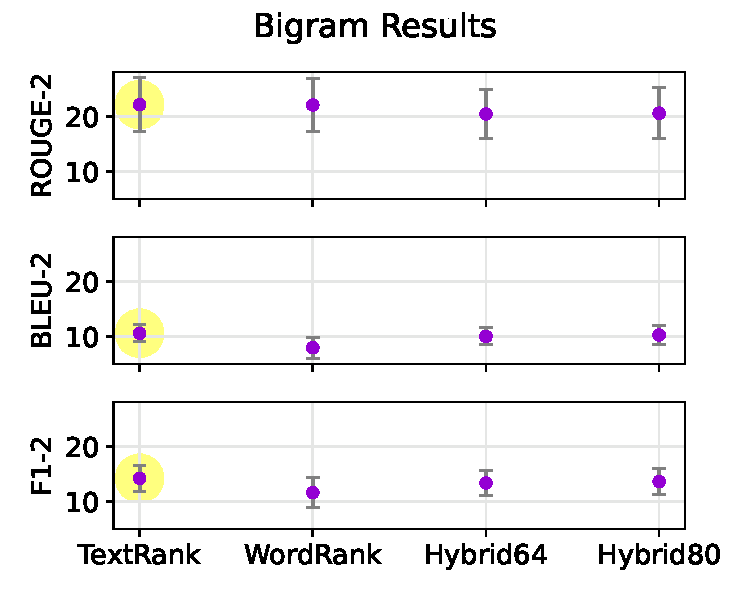
\includegraphics[scale = 0.5]{../figures/bigrams.pdf}
\caption{ROUGE, BLEU, and F1 score of bigrams between the human-written and generated summaries.\label{fig:bi}}
\end{figure}

\begin{figure}[!h]
\centering
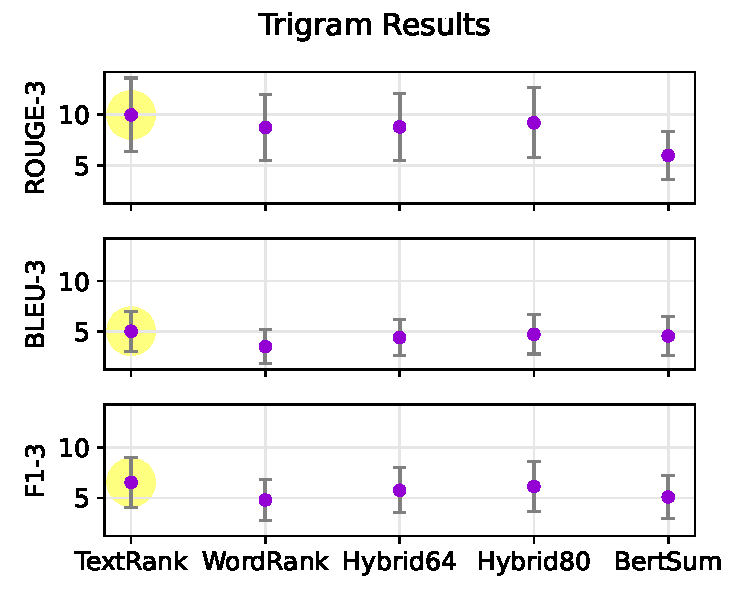
\includegraphics[scale = 0.5]{../figures/trigrams.pdf}
\caption{ROUGE, BLEU, and F1 score of trigrams between the human-written and generated summaries.\label{fig:tri}}
\end{figure}

\begin{table*}[!h]
\centering
\begin{tabular}{l|llll}
\hline
&\textbf{TextRank} & \textbf{WordRank} & \textbf{Hybrid64} & \textbf{Hybrid80} \\
\hline
ROUGE\_1 & 57.4 & \textbf{60.1} & 57.2 & 57.1\\
ROUGE\_2 & \textbf{21.2} & 20.3 & 19.9 & 20.3\\
ROUGE\_3 & \textbf{10.0} & 8.7 & 8.8 & 9.2\\
BLEU\_1 & \textbf{27.0} & 20.8 & 26.7 & 26.8\\
BLEU\_2 & \textbf{10.1} & 7.3 & 9.5 & 9.8\\
BLEU\_3 & \textbf{5.0} & 3.5 & 4.4 & 4.7\\
F1\_1 & \textbf{36.0} & 30.3 & 35.7 & 35.9\\
F1\_2 & \textbf{13.4} & 10.4 & 12.6 & 12.9\\
F1\_3  & \textbf{6.5} & 4.8 & 5.8 & 6.1\\
\hline
\end{tabular}

\caption{\label{tab:means}
Mean values of the ROUGE, BLEU, and F1 metrics for unigrams, bigrams, and trigrams yielded by TextRank, WordRank, Hybrid64, and Hybrid80 methods.
}
\end{table*}

\begin{table*}[!h]
\centering
\begin{tabular}{l|llll}
\hline
&\textbf{TextRank} & \textbf{WordRank} & \textbf{Hybrid64} & \textbf{Hybrid80} \\
\hline
ROUGE\_1 & 4.7 & 4.1 & 4.1 & 4.3\\
ROUGE\_2 & 4.9 & 4.6 & 4.4 & 4.7\\
ROUGE\_3 & 3.7 & 3.2 & 3.3 & 3.5\\
BLEU\_1 & 3.7 & 3.2 & 3.1 & 3.2\\
BLEU\_2 & 2.7 & 2.2 & 2.3 & 2.5\\
BLEU\_3 & 2.0 & 1.7 & 1.8 & 1.9\\
F1\_1 &  3.7 & 3.6 & 3.2 & 3.3\\
F1\_2 & 3.2 & 2.8 & 2.9 & 3.1\\
F1\_3  & 2.5 & 2.0 & 2.2 & 2.4\\
\hline
\end{tabular}
\caption{\label{tab:mors}
Margins of error values of the ROUGE, BLEU, and F1 metrics for unigrams, bigrams, and trigrams yielded by TextRank, WordRank, Hybrid64, and Hybrid80 methods.
}
\end{table*}


\begin{table*}[!h]
\centering
\begin{tabular}{l|llll}
\hline
&\textbf{TextRank} & \textbf{WordRank} & \textbf{Hybrid64} & \textbf{Hybrid80} \\
\hline
Running time (min) & 1 & 16 & 16 & 16\\
\hline
\end{tabular}
\caption{\label{tab:time}
Running time (min) of all four algorithms considered in this project.
}
\end{table*}


\section{Discussion}

\section{Conclusion}




\section{Preamble}
\begin{table*}
\centering
\begin{tabular}{lll}
\hline
\textbf{Output} & \textbf{natbib command} & \textbf{Old ACL-style command}\\
\hline
\citep{ct1965} & \verb|\citep| & \verb|\cite| \\
\citealp{ct1965} & \verb|\citealp| & no equivalent \\
\citet{ct1965} & \verb|\citet| & \verb|\newcite| \\
\citeyearpar{ct1965} & \verb|\citeyearpar| & \verb|\shortcite| \\
\citeposs{ct1965} & \verb|\citeposs| & no equivalent \\
\citep[FFT;][]{ct1965} &  \verb|\citep[FFT;][]| & no equivalent\\
\hline
\end{tabular}
\caption{\label{citation-guide}
Citation commands supported by the style file.
The style is based on the natbib package and supports all natbib citation commands.
It also supports commands defined in previous ACL style files for compatibility.
}
\end{table*}






Table~\ref{citation-guide} shows the syntax supported by the style files.
We encourage you to use the natbib styles.
You can use the command \verb|\citet| (cite in text) to get ``author (year)'' citations, like this citation to a paper by \citet{Gusfield:97}.
You can use the command \verb|\citep| (cite in parentheses) to get ``(author, year)'' citations \citep{Gusfield:97}.
You can use the command \verb|\citealp| (alternative cite without parentheses) to get ``author, year'' citations, which is useful for using citations within parentheses (e.g. \citealp{Gusfield:97}).




% Entries for the entire Anthology, followed by custom entries
\bibliography{custom}
\bibliographystyle{acl_natbib}


\end{document}
